\chapter*{3 Versuchsdurchführung und Auswertung}
\addcontentsline{toc}{chapter}{3 Versuchsdurchführung und Auswertung}
\setcounter{chapter}{3}
\setcounter{section}{0}
\setcounter{subsection}{0}

\section{Versuch 1 - Bestimmung der spezifischen Wärme des Wasser auf mechanischen Wege}
	
	\subsection{Aufbau/Theorie}
	\begin{figure}[ht]
		\label{fig:abb1}
		   \begin{center}
		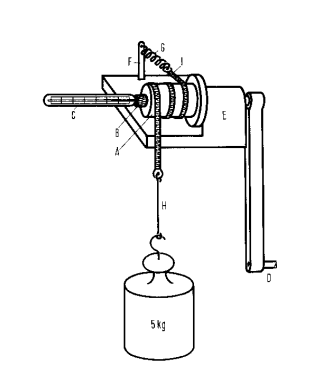
\includegraphics[width=0.2\textwidth]{bilder/Schuerholz.png}
		\caption{Schürholzapparatur}
	\end{center}
	\end{figure}
		Die spezifische Wärmeänderung eines Stoffes charakterisiert die quantitativen Veränderungen der inneren Energie pro Masseneinheit, die auftreten, wenn sich die Temperatur des Stoffes entsprechend ändert. Die Spezifische Wärmekapazität misst also die Fähigkeit eines Materials, Wärmeenergie zu absorbieren oder abzugeben und dabei die Temperatur zu verändern. Diese versuchen wir im folgenden mit der Abbildung \ref{fig:abb1} zu bestimmen. Dazu wird das Kalorimeter mit Wasser befüllt und dann durch Reibung des Fadens Wärme erzeugt die in das Kalorimeter übergeht. Aus der Differenz der Wärme des Wasser im Kalorimeter lässt sich nun die Wärmeenergie bestimmen welche der Reibungsenergie entsprechen sollte.
		Dafür nutzen wir folgende Formeln:
		
		Reibungsenergie:
		$$W_{r} = F_{r} \cdot 2\pi \cdot r \cdot n$$
		
		Wärmeenergie:
		$$Q_{r} =  (\Gamma_{K} + m_{\omega}c_{\omega}) \cdot \Delta T$$
		
		Setzt man diese nun gleich lässt sich die spezifische Wärmekapazität von dem Wasser berechnen:
		$$G \cdot 2\pi \cdot r \cdot n = (m_{K}c_{K} + m_{\omega}c_{\omega}) \cdot \Delta T$$
		$$ \Rightarrow c_{\omega} = \frac{\frac{W_{r}}{\Delta T} - m_{K}c_{K}}{m_{\omega}}$$		
		
		Dies werden wir nun im folgenden Versuch durchführen.
		
	    \subsection{Versuchsdurchführung}
		\textbf{\textcolor{red}{TODO}}
	
  
    \subsection{Ergebnisse}

        \begin{table}[H]
            \centering
            \begin{tabular}{|l|l|l|l|}
                \hline
                & Anzahl der Umdrehungen $n$ & Temperatur in °C & $\Delta$ Temperatur in °C\\
                \hline
                $n = 0$ & - & -& -\\
                \hline
                $n = 50$ & - & - & -\\
                \hline
                $n = 100$ & - & - & -\\
                \hline
                $n = 150$ & - & - & -\\
                \hline
                $n = 200$ & - & - & -\\
                \hline
                $n = 250$ & - & - & -\\
                \hline
            \end{tabular}
        \end{table}

Der ermittelte Wert für die spezifische Wärmeänderung $c_{ermittelt\omega} = ? \frac{J}{kgK}$ weicht leicht vom Literaturwert für die spezifische Wärmekapazität von Wasser $c_{Lit\omega} = 4190 \frac{J}{kgK}$ ab. Diese geringfügige Diskrepanz könnte auf einzelne Messungenauigkeiten zurückgeführt werden, die sich auf das Endergebnis auswirken.
Darüber hinaus ist anzumerken, dass eine hundertprozentige Energieerhaltung bei der Umwandlung von Reibungsenergie in Wärmeenergie in der Praxis nicht realisierbar ist. Das kann zu weiteren Abweichungen zwischen dem gemessenen und dem theoretisch erwarteten Wert führen. Die Verfälschung des genauen Ergebnisses ist daher teilweise auf die inhärente Unvollkommenheit praktischer Energieumwandlungsprozesse zurückzuführen. 


\section{Versuch 2 - Vgl. verschiedener Temperaturmessmethoden}
    \subsection{Theorie Thermoelement/Widerstandsthermometer und Strahlungsthermometer}
    \subsubsection*{Thermoelement:}
    	\begin{figure}[ht]
    	\label{fig:abb2}
    	\begin{center}
    		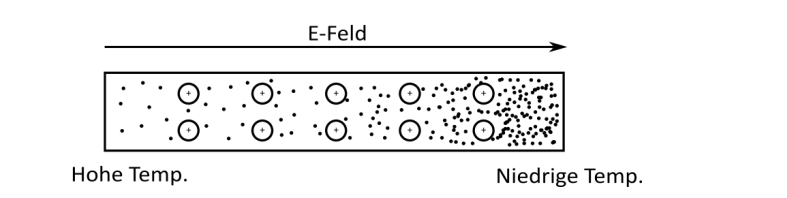
\includegraphics[width=0.5\textwidth]{bilder/Seebeck-Effekt.png}
    		\caption{Der Seebeck-Effekt vereinfacht dargestellt.}
    	\end{center}
    \end{figure}
    Durch die Anwendung eines Thermoelements ist es möglich, die Temperatur eines Stoffes zu bestimmen. Bei einem elektrischen Leiter, dessen zwei Enden unterschiedlichen Temperaturen ausgesetzt sind, entsteht aufgrund des Seebeck-Effekts eine elektrische Spannung. Dieser Effekt basiert darauf, dass Elektronen am wärmeren Ende eine höhere kinetische Energie aufweisen, wie in Abbildung \ref{fig:abb2} illustriert. Im Gegensatz dazu besitzen Elektronen am kälteren Ende eine geringere Bewegungsenergie, was zu einer höheren Elektronendichte führt. Der resultierende Unterschied in der Elektronendichte führt zu einer messbaren elektrischen Spannung.
    
   Die Höhe der gemessenen Spannung korreliert direkt mit der Größe des Temperaturunterschieds zwischen den beiden Enden des Leiters. Ein größerer Temperaturunterschied führt also zu einer höheren Spannung, die durch das Thermoelement erfasst werden kann.
   \subsubsection*{Widerstandsthermometer:}
   Das Widerstandsthermometer besteht lediglich aus einem Widerstand welcher an einem Multimeter angeschlossen ist. Taucht man diesen in die zu messende Flüssigkeit und der angezeigte Widerstand liegt zwischen 2 Werten in der Tabelle, welche in der Anleitung angehängt ist, so lässt sich durch Interpolation ein genauerer Temperaturwert bestimmen. Sei R der Widerstand und und T die Temperatur so lässt sich mit folgender Formel die gemessene Temperatur berechnen.
   $$T = T_{1} + \frac{R - R_{1}}{R_{2} - R_{1}} \cdot \Delta T$$
   \subsubsection*{Strahlungsthermometer}
   Ein Strahlungsthermometer misst die Temperatur eines Objekts, indem es die von ihm emittierte Infrarotstrahlung erfasst. Die gemessene Temperatur steht in direktem Zusammenhang mit der Temperatur des Objekts, sowie dem Abstand des Objekts zum Thermometer.  Der Abstand sollte also $\leq$ 10cm zum Objekt liegen um störende Strahlen vom Rand oder der Umgebung zu vermeiden. 
    \subsection{Versuchsaufbau und -durchführung}
     Kallibrieren

		\textbf{\textcolor{red}{TODO}}
    \subsection{Ergebnisse}
      

\section{Versuch 3 - Bestimmung der spezifischen Wärme von Wasser auf elektrischem Wege}
    \subsection{Theorie}
    
        	\begin{figure}[ht]
    	\label{fig:abb3}
    	\begin{center}
    		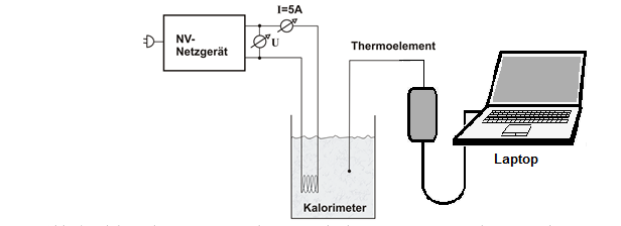
\includegraphics[width=0.6\textwidth]{bilder/Elektrisch.png}
    		\caption{Auffbau Versuch 3.}
    	\end{center}
    \end{figure}
    Die spezifische Wärmekapazität des Wassers kann auch bestimmt werden, indem man mit Hilfe der
    Joulschen Wärme, die in einem stromdurchflossenen Leiter entsteht, eine definierte Wassermenge
    erwärmt und deren Temperaturerhöhung misst, siehe Abbildung \ref{fig:abb3}. Hierzu wird eine Heizspirale ins Kalorimeter
    eingebracht, die mit einem Niedervolt-Netzgerät betrieben wird. Während des Aufheizvorgangs (5
    Minuten) werden Strom (ca. 5 A) und Spannung (ca. 10V) mit einem Amperemeter bzw. einem
    Voltmeter gemessen (wird direkt vom Gerät angezeigt). 
   Da wir von einem abgeschlossenen System ausgehen, können die zugeführte und aufgenommene
   Energie gleichgesetzt werden. Stellt man dann noch die entstandene Gleichung nach dem
   gewünschten Wert um so kann die spezifische Wärmekapazität von Wasser bestimmt werden.
   
   \noindent Hierzu benötigen die aufgenommen Wärmemenge:
   $$\Delta Q = (C_{K} + m_{Wasser}c{Wasser} ) \cdot \Delta T$$
   und die aufgewendete elektrische Arbeit:
   $$\Delta W =  U \cdot I \cdot \Delta t$$
   
   Nun lässt es sich Gleichsetzen und nach $c_{Wasser}$ umstellen:
   $$c_{Wasser} = \frac{UI\Delta t - C_{K}\Delta T}{m_{Wasser} \Delta T}$$
    \subsection{Versuchsdurchführung}

        		\textbf{\textcolor{red}{TODO}}
    \subsection{Ergebnisse}



        \begin{table}[H]
            \centering
            \begin{tabular}{|l|l|l|l|l|l|l|}
                \hline
                $G_{B}$in Kg & $G_{W}$ in Kg & Strom in A & Spannung in Volt  & $T_{1}$ in °C & $T_{2}$ in °C & $\Delta T$ in °C \\
                \hline
                -& - & - & - & - & - & - \\
                \hline
    
            \end{tabular}
        \end{table}

\section{Versuch 4 - Spezifische Wärmekapazität fester Körper}
	    \subsection{Theorie}
	Die spezifische Wärmekapazität fester Körper wird mittels der Mischungsmethode bestimmt, indem ein Probekörper der Masse $m_{1}$ auf die Temperatur von siedendem Wasser erhitzt wird und anschließend in ein Kalorimeter mit Wasser der Masse $m_{2}$ und Anfangstemperatur $T_{2}$ gebracht wird. Die Entwicklung der Mischtemperatur $T_{misch}$ aufgezeichnet wird aufgezeichnet und draus die Wärmekapazität des Körpers berechnet.
	
	Dazu benötigt man die vom Körper abgegeben Wärmeenergie:
	$$\Delta Q_{1} = m_{1}c_{1} \cdot (T_{1} - T_{misch})$$
	wobei $c_{1}$ die spezifische Wärmekapazität ist die berechnet werden soll. Die im Kalorimeter aufgenommen Wärmemenge lässt sich mit:
	$$\Delta Q_{2} = (C_{K} + m_{2}c_{Wasser}) \cdot (T_{misch} - T_{2})$$
	berechnen.
	
	Da wir von einem abgeschlossenen System ausgehen lässt sich $c_{1}$ durch Gleichsetzen von $Q_{1} = Q_{2}$ und umstellen tatsächlich berechnen:
	$$c_{1} = \frac{(C_{K} +m_{2}c_{Wasser}) \cdot (T_{misch} - T_{2})}{m_{1} \cdot (T_{1} - T_{misch})}$$
	
	Der Aufbau sieht in etwa so aus:
	       	\begin{figure}[ht]
		\label{fig:abb4}
		\begin{center}
			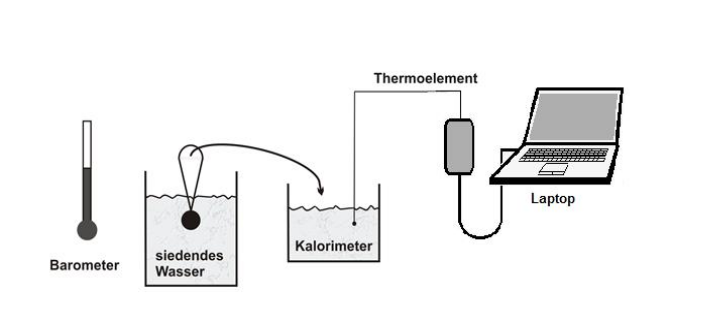
\includegraphics[width=0.6\textwidth]{bilder/Fest.png}
			\caption{Auffbau Versuch 4.}
		\end{center}
	\end{figure}
    \subsection{Versuchsdurchführung}


    		\textbf{\textcolor{red}{TODO}}
    \subsection{Ergebnisse}



        \begin{table}[H]
            \centering
            \begin{tabular}{|l|l|l|l|}
                \hline
                Metallart & $\Delta T_{1}$ & $\Delta T_{2}$ & \o $ \Delta T_{3}$\\
                \hline
                Eisen& - & - & - \\
                \hline
                Messing & - & - & - \\
                \hline
                Aluminium& - & - & - \\
                \hline
            \end{tabular}
        \end{table}
        
        \begin{table}[H]
        	\centering
        	\begin{tabular}{|l|l|l|l|}
        		\hline
        		Metallart & Literaturwert $(\frac{J}{KgK})$ & Berechnet $(\frac{J}{KgK})$ & Abweichung $(\frac{J}{KgK})$ \\
        		\hline
        		Eisen& - & - & - \\
        		\hline
        		Messing & - & - & - \\
        		\hline
        		Aluminium& - & - & - \\
        		\hline
        	\end{tabular}
        \end{table}



\section{Versuch 5 - Latente Wärme - die spezifische Schmelzwärme von Wassser}
    \subsection{Theorie}
    \subsection{Versuchsaufbau und -durchführung}
        

    
    \subsection{Ergebnisse}

        Die Messwerte sind in der folgenden Tabelle aufgelistet:

        \begin{table}[H]
            \centering
            \begin{tabular}{|l|l|l|}
                \hline
                Abstand $a_{1}$ & Abstand $L$ & Dicke (berechnet)\\
                \hline
                $2,3 \pm 0,1\ \mathrm{cm}$ & $150 \pm 0,1\ \mathrm{cm}$ & $82,5\ \mathrm{\mu m}$\\
                \hline
            \end{tabular}
        \end{table}

